\problemname{Studschiffret}

Fretchif har hittat på ett revolutionärt chiffer som ingen kommer kunna lösa! Så här går det till: Man väljer en sträng att kryptera och två heltal $N$ och $M$. Sedan ritar man upp ett rutnät med $N$ rader och $M$ kolumner. Därefter börjar man skriva ut strängen man krypterar en bokstav i taget snett nedåt till höger från översta vänstra hörnet. Om vi numrerar kolumnerna från vänster till höger $1$ till $M$, och raderna uppifrån och ned $1$ till $N$ så hamnar första bokstaven hamnar på position $(1,1)$, andra på $(2,2)$, tredje på $(3,3)$ och så vidare. När man kommer till en av rutnätets väggar, så låter man ”bokstavsstrålen” studsa på väggen (se exempelförklaringen). Ifall man vid något tillfälle hamnar på en ruta som det redan står en bokstav i, så tar bokstaven man skulle skrivit och skriver den i nästa lediga ruta man kommer till istället. När alla bokstäver i strängen som krypteras är slut så läser man av rutnätet rad för rad, och det blir det krypterade meddelandet. 
\\ \\
Givet ett meddelande som Fretchif krypterat med studschiffret, och givet storleken på rutnätet som användes, skriv ut orginalmeddelandet.
\\ \\
Notera att vissa meddelanden inte går att kryptera med vissa storlekar på rutnät, då det är möjligt att man aldrig kommer till någon ny ledig ruta men fortfarande har bokstäver kvar att placera ut. Här är det dock garanterat att det inte hände när Fretchif krypterade strängen.

\section*{Exempelförklaring}
Säg att strängen vi ska kryptera är \texttt{ABCDEFGHIKLMNOPQRST}, och att rutnätet har storlek $6 \times 13$.
Så här ser rutnätet ut vid olika tidspunkter i krypteringen: \hspace{25cm}
\begin{figure}[!h]
  \centering
      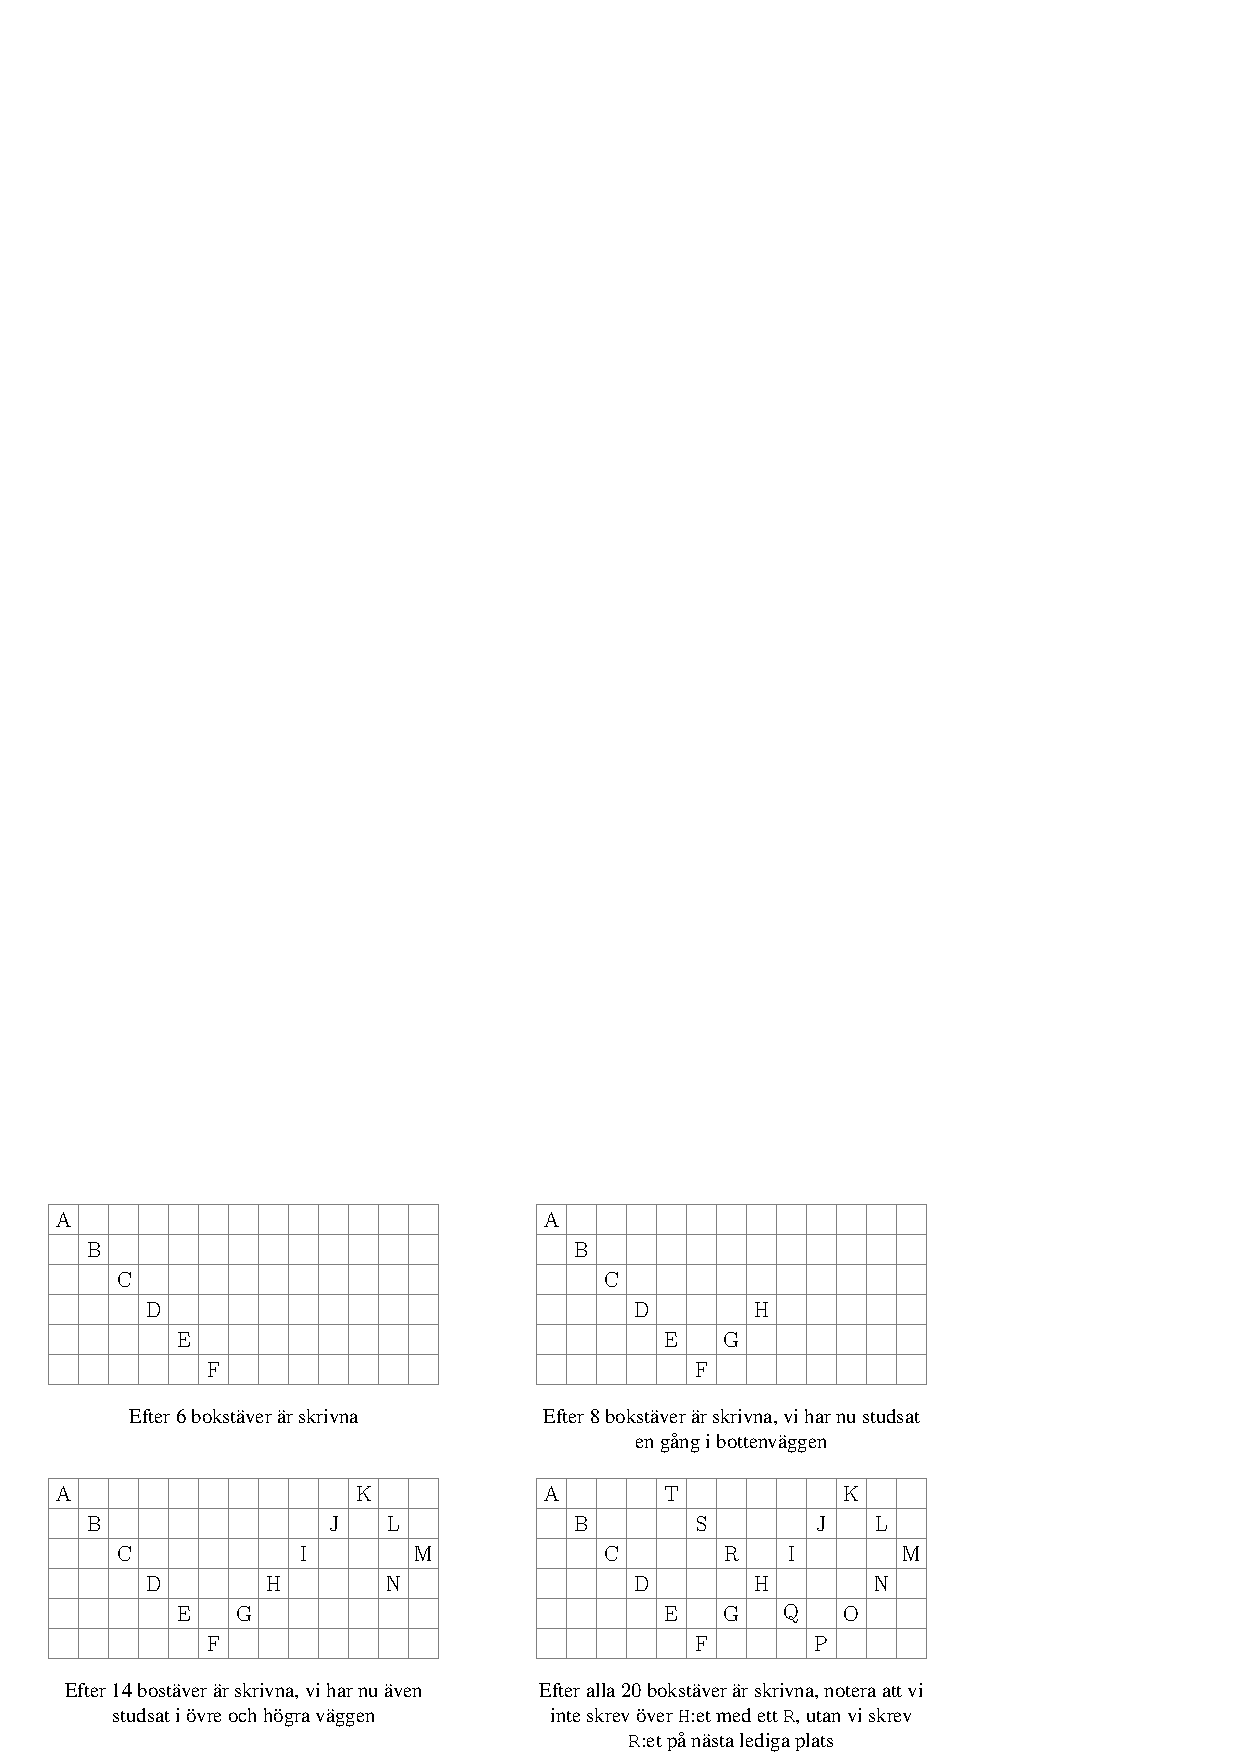
\includegraphics[width=1\textwidth]{grids.pdf}
\end{figure}

I det här exemplet blir alltså det krypterade meddelandet \texttt{ATKBSJLCRIMDHNEGQOFP}. Exempel 2 är att avkoda \texttt{ATKBSJLCRIMDHNEGQOFP}, vilket då avkodas till \texttt{ABCDEFGHIKLMNOPQRST}.

\section*{Indata}
På första raden står två heltal $2 \leq N \leq 20$ och $2 \leq M \leq 20$, antalet rader och kolumner i rutnätet.  
På andra raden står en sträng med $K$ bokstäver ($1 \leq K \leq 30$), det krypterade meddelandet. Meddelandet består endast av bokstäverna \texttt{A} till \texttt{Z} och alla bokstäver är stora.
Det är garanterat att det finns en möjlig ursprungssträng som ger denna chiffertext.

\section*{Utdata}
Programmet ska skriva ut en rad med en sträng: orginalmeddelandet, så som det såg ut innan det krypterades.

\section*{Poängsättning}
För testfall värda $20$ poäng gäller att $N=2$ och att bokstavsstrålen aldrig studsar på högra väggen\\
För testfall värda $40$ poäng gäller att bokstavsstrålen aldrig studsar på högra väggen\\
